
  
\documentclass[journal,12pt,twocolumn]{IEEEtran}

\usepackage{setspace}
\usepackage{gensymb}
\singlespacing
\usepackage[cmex10]{amsmath}

\usepackage{amsthm}
\usepackage{commath}
\usepackage{mathrsfs}
\usepackage{txfonts}
\usepackage{stfloats}
\usepackage{bm}
\usepackage{cite}
\usepackage{cases}
\usepackage{subfig}

\usepackage{longtable}
\usepackage{multirow}

\usepackage{enumitem}
\usepackage{mathtools}
\usepackage{steinmetz}
\usepackage{tikz}
\usepackage{circuitikz}
\usepackage{verbatim}
\usepackage{tfrupee}
\usepackage[breaklinks=true]{hyperref}
\usepackage{graphicx}
\usepackage{tkz-euclide}

\usetikzlibrary{calc,math}
\usepackage{listings}
    \usepackage{color}                                            %%
    \usepackage{array}                                            %%
    \usepackage{longtable}                                        %%
    \usepackage{calc}                                             %%
    \usepackage{multirow}                                         %%
    \usepackage{hhline}                                           %%
    \usepackage{ifthen}                                           %%
    \usepackage{lscape}     
\usepackage{multicol}
\usepackage{chngcntr}

\DeclareMathOperator*{\Res}{Res}

\renewcommand\thesection{\arabic{section}}
\renewcommand\thesubsection{\thesection.\arabic{subsection}}
\renewcommand\thesubsubsection{\thesubsection.\arabic{subsubsection}}

\renewcommand\thesectiondis{\arabic{section}}
\renewcommand\thesubsectiondis{\thesectiondis.\arabic{subsection}}
\renewcommand\thesubsubsectiondis{\thesubsectiondis.\arabic{subsubsection}}


\hyphenation{op-tical net-works semi-conduc-tor}
\def\inputGnumericTable{}                                 %%

\lstset{
%language=C,
frame=single, 
breaklines=true,
columns=fullflexible
}
\begin{document}

\newcommand{\BEQA}{\begin{eqnarray}}
\newcommand{\EEQA}{\end{eqnarray}}
\newcommand{\define}{\stackrel{\triangle}{=}}
\bibliographystyle{IEEEtran}
\raggedbottom
\setlength{\parindent}{0pt}
\providecommand{\mbf}{\mathbf}
\providecommand{\pr}[1]{\ensuremath{\Pr\left(#1\right)}}
\providecommand{\qfunc}[1]{\ensuremath{Q\left(#1\right)}}
\providecommand{\sbrak}[1]{\ensuremath{{}\left[#1\right]}}
\providecommand{\lsbrak}[1]{\ensuremath{{}\left[#1\right.}}
\providecommand{\rsbrak}[1]{\ensuremath{{}\left.#1\right]}}
\providecommand{\brak}[1]{\ensuremath{\left(#1\right)}}
\providecommand{\lbrak}[1]{\ensuremath{\left(#1\right.}}
\providecommand{\rbrak}[1]{\ensuremath{\left.#1\right)}}
\providecommand{\cbrak}[1]{\ensuremath{\left\{#1\right\}}}
\providecommand{\lcbrak}[1]{\ensuremath{\left\{#1\right.}}
\providecommand{\rcbrak}[1]{\ensuremath{\left.#1\right\}}}
\theoremstyle{remark}
\newtheorem{rem}{Remark}
\newcommand{\sgn}{\mathop{\mathrm{sgn}}}
\providecommand{\abs}[1]{\vert#1\vert}
\providecommand{\res}[1]{\Res\displaylimits_{#1}} 
\providecommand{\norm}[1]{\lVert#1\rVert}
%\providecommand{\norm}[1]{\lVert#1\rVert}
\providecommand{\mtx}[1]{\mathbf{#1}}
\providecommand{\mean}[1]{E[ #1 ]}
\providecommand{\fourier}{\overset{\mathcal{F}}{ \rightleftharpoons}}
%\providecommand{\hilbert}{\overset{\mathcal{H}}{ \rightleftharpoons}}
\providecommand{\system}{\overset{\mathcal{H}}{ \longleftrightarrow}}
	%\newcommand{\solution}[2]{\textbf{Solution:}{#1}}
\newcommand{\solution}{\noindent \textbf{Solution: }}
\newcommand{\cosec}{\,\text{cosec}\,}
\providecommand{\dec}[2]{\ensuremath{\overset{#1}{\underset{#2}{\gtrless}}}}
\newcommand{\myvec}[1]{\ensuremath{\begin{pmatrix}#1\end{pmatrix}}}
\newcommand{\mydet}[1]{\ensuremath{\begin{vmatrix}#1\end{vmatrix}}}
\numberwithin{equation}{subsection}
\makeatletter
\@addtoreset{figure}{problem}
\makeatother
\let\StandardTheFigure\thefigure
\let\vec\mathbf
\renewcommand{\thefigure}{\theproblem}
\def\putbox#1#2#3{\makebox[0in][l]{\makebox[#1][l]{}\raisebox{\baselineskip}[0in][0in]{\raisebox{#2}[0in][0in]{#3}}}}
     \def\rightbox#1{\makebox[0in][r]{#1}}
     \def\centbox#1{\makebox[0in]{#1}}
     \def\topbox#1{\raisebox{-\baselineskip}[0in][0in]{#1}}
     \def\midbox#1{\raisebox{-0.5\baselineskip}[0in][0in]{#1}}
\vspace{3cm}
\title{Assignment 3}
\author{Adarsh Sai - AI20BTECH11001}
\maketitle
\newpage
\bigskip
\renewcommand{\thefigure}{\theenumi}
\renewcommand{\thetable}{\theenumi}
Download all python codes from 
\begin{lstlisting}
https://github.com/Adarsh541/EE3900/blob/main/Assignment2/codes/Assignment3.py
\end{lstlisting}

%
Download latex-tikz codes from 
%
\begin{lstlisting}
https://github.com/Adarsh541/EE3900/blob/main/Assignment3/Assignment3.tex
\end{lstlisting}
\section{Problem(Construction Q2.3)}
Draw JUMP with $JU = 3.5$, $UM = 4$, $MP = 5$, $PJ = 4.5$ and $PU = 6.5$
\section{Solution}
The vertices $\vec{P}$ and $\vec{U}$ are
\begin{align}
    \vec{P} = \myvec{0\\0}, \vec{U} = \myvec{PU\\0} = \myvec{6.5\\0
    }
\end{align}
Let $\angle{UPM} = \theta_1$ and  $\angle{JPU} = \theta_2$
\begin{align}
    \cos{\theta_1} &= \frac{5^2+6.5^2-4^2}{2(5)(6.5)}\\
    &=0.7884\\
    \implies \theta_1 &= 37.958^{\circ}\\
    \sin{\theta_1} &= 0.615\\
    \cos{\theta_2} &= \frac{6.5^2+4.5^2-3.5^2}{2(6.5)(4.5)}\\
    &= 0.8589\\
    \implies \theta_2 &= 30.798^{\circ}\\
    \sin{\theta_2} &= 0.512
\end{align}
Now, the vertices $\vec{M}$ and $\vec{J}$ can be expressed in polar coordinate form as
\begin{align}
    \vec{M} &= 5\myvec{\cos{\theta_1}\\\sin{\theta_1}}\\
    &= \myvec{3.942\\3.075}\\
    \vec{J} &= 4.5\myvec{\cos{\theta_2}\\-\sin{\theta_2}}\\
    &= \myvec{3.865\\-2.304}
\end{align}

%%%%%%%%
\begin{tikzpicture}[scale=1]



%Marking coordiantes
\coordinate [label=above:$M$] (M) at (3.942,3.075);
\coordinate [label=below:$J$] (J) at (3.865,-2.304);
\coordinate [label=right:$U$] (U) at (6.5,0);
\coordinate [label=left:$P$] (P) at (0,0);

%Drawing triangle ABC
\draw (P) -- node[above] {6.5} (U) -- node[above] {4} (M) -- node[above] {5} (P) -- node[below] {4.5}(J) -- node[below] {3.5} (U);


%Drawing and marking angles
\tkzMarkAngle[fill=orange!40,size=0.5cm,mark=](U,P,M)
\tkzLabelAngle[pos=0.85](U,P,M){$\theta_1$}
\tkzMarkAngle[fill=orange!40,size=0.9cm,mark=](J,P,U)
\tkzLabelAngle[pos=1.3](J,P,U){$\theta_2$}
\end{tikzpicture}

\begin{figure}[!h]
 \centering
 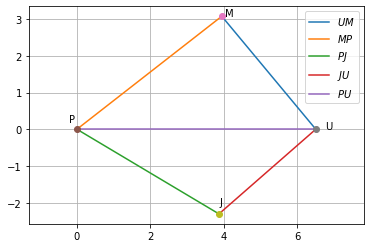
\includegraphics[width=\columnwidth]{Assignment3.png}
 \caption{Plot using python}
 \label{plot}
\end{figure}
\end{document}

